\chapter{Technologien zur Erstellung von 3D Computergrafiken}
\label{chap_technologien}
Dieses Kapitel bietet einen Überblick über die Technologielandschaft zur Erstellung von 3D Computergrafiken. Konkret wird auf populäre Spiele Engines wie Unity, Godot sowie Unreal Engine eingegangen. Nebst den Engines werden auch verschiedene Frameworks wie ThreeJS, CelsiumJs sowie sokol thematisiert. Zu guter letzt wird noch auf immersive Technologien wie \acrshort{VR} sowie \acrshort{CAVE} eingegangen.

\section{Engines}
Engines sind umfassende Programme, welche das Erstellen von 3D Computergrafiken und insbesondere Videospielen für jedermann zugänglich machen. Anders als Frameworks beinhalten diese integrierte Editoren, welche das Erstellen von Spielwelten und interaktiven Erlebnissen unterstützen, sowie fertige Komponenten für komplette Physik- und Audiosysteme anbieten. Wie bei normalen Programmen gibt es auch bei Spiele Engines kostenlose und kostenpflichtige Varianten. Nachfolgend wird auf die populärsten 3D-fokussierten Engines in beiden Bereichen eingegangen.  

\subsection{Unity Engine}
Rückblickend auf das Jahr 2024 bezogen ist die Unity Engine ist die meist genutzte Spiele Engine für kleinere bis mittelgrosse 3D Erlebnisse (siehe Abbildung \ref{fig_nutzung_spiele_engines}). Unity gehört zu den kostenpflichtigen Spiele Engines und unterstützt rund 20 verschiedene Plattformen. Angefangen bei den klassischen Desktop-Betriebssystemen wie MacOS, Linux und Windows über Webbrowser bis zu verschiedenen Spielekonsolen und VR-Headsets \parencite{unity_platform_support_2025}.
\begin{figure}[H]
    \caption{Übersicht Nutzung Spiele Engine nach Spielgrösse \parencite[S. 7]{vgi_report_2025}}
    \includegraphics[width=.5\linewidth]{content/00_assets/uebersicht_nutzung_spielengines.png}
    \label{fig_nutzung_spiele_engines}
\end{figure}

Die Spiele selbst werden in Unity innerhalb des Unity-Editors (siehe Abbildung \ref{fig_unity_editor}) und mithilfe der Programmiersprache C-Sharp entwickelt. 
\begin{figure}[H]
    \caption{Unity Editor \parencite{unity_editor_2019}}
    \includegraphics[width=.5\linewidth]{content/00_assets/unity_editor.jpg}
    \label{fig_unity_editor}
\end{figure}

Je nach Funktionsumfang gibt es verschiedene Lizenzmodelle bei Unity. Das Lizenzmodell ist jedoch nicht nur vom Funktionsumfang, sondern auch vom Jahreseinkommen (siehe Tabelle \ref{table_unity_preise}). Nebst den unten aufgeführten Lizenzen gibt es zudem noch eine Industry-Lizenz welche beim Erstellen von industriellen Anwendungen erworben werden muss (Preis auf Anfrage).
\begin{table}[H]
    \caption{Lizenzmodell Unity Engine mit Jahreskosten abhängig vom Jahreseinkommen \parencite{unity_preise_2025}}
    \begin{tabularx}{\textwidth} {
        >{\raggedright\arraybackslash}X 
        >{\raggedright\arraybackslash}X
        >{\raggedright\arraybackslash}X}
            \hline
            \textbf{Lizenzmodell} & {Jahreseinkommen} & {Jahreskosten}  \\
            \hline
            Personal & weniger als 200'000 USD & {Gratis}\\
            Pro & zwischen 200'000 USD und 25'000'000 USD & 2'220 USD pro Nutzer \\
            Enterprise & mehr als 25'000'000 USD &  auf Anfrage \\
            \hline
    \end{tabularx}
    \bigbreak
    \label{table_unity_preise}
\end{table}

\subsection{Unreal Engine}
Über die Jahre haben viele Spielentwicklungsstudios bekannt gegeben, dass sie ihre eigene In-House Engine durch die Unreal Engine ersetzen werden \parencite[S. 11]{vgi_report_2025}. Unreal zeichnet sich durch die beeindruckenden visuellen Effekte aus. Unreal Engine wird jedoch nicht nur zur Entwicklung von Videospielen eingesetzt, sondern auch im Rahmen von Filmproduktionen sowie Architekturvisualisierungen (siehe Abbildung \ref{fig_unreal_engine_architektur}). Insbesondere in der Achitekturvisualisiserung werden auch verschiedene gängige Datenformate wie \acrfull{BIM} unterstützt \parencite{unreal_engine_architektur_2025}. Unreal Engine gehört ebenfalls zu den kommerziellen Spiele Engines. Beim Lizenzmodell wird zwischen zwei verschiedenen Kategorien unterschieden. Werden mit der Videospiele erstellt, so ist die Engine bis zu einem Umsatz von 1'000'000 USD komplett kostenlos. Danach müssen jweiles 5\% des Gewinns als Lizenzkosten abgegeben werden. Werden hingegen keine Videospiele sondern kommerzielle Produkte erstellt, so fallen nach der ersten Million Umsatz rund 1'800 USD pro Nutzer im Jahr als Lizenzgebühren an \parencite{unreal_engine_lizenzkosten_2025}. 
\begin{figure}[H]
    \caption{Unreal Engine Achitektur Visualisierung \parencite{unreal_engine_architektur_2025}}
    \includegraphics[width=.5\linewidth]{content/00_assets/unreal_engine_achitektur.png}
    \label{fig_unreal_engine_architektur}
\end{figure}

Unreal Engine selbst bietet dem Nutzer ebenfalls einen integrierten Editor sowie zahlreiche Tools um die Erstellung von immersiven Erlebnissen zu vereinfachen. Beispielsweise können mithilfe des Tools World Partitioning riesige 3D-Welten erstellt werden. Hierbei wird die Welt in ein Gitternetz unterteilt und die einzelnen Teilbereiche werden, wenn sich der Nutzer durch die Welt bewegt, dynamisch nachgeladen \parencite{unreal_engine_2025}. Auch beim Erstellen der notwendigen 3D Modelle unterstützt Untreal Engine mit diversen Tools. Quixel Megascan erlaubt das Integrieren von 3D Modellen mithilfe von fotogrammetrischen Verfahren sowie die Nutzung von hochauflösenden Texturen \parencite{unreal_engine_quixel_2025}. Anders als in Unity wird die systemnahe Programmiersprache C++ in Kombination mit der visuellen Scriptsprache Blueprints verwendet.

\subsection{Godot Engine}
Die Godot Engine ist Open Source, frei zugängliche und kostenlos. Godot ist ebenfalls sehr leichtgewichtig und benötigt nur rund 200MB - 1.5GB in der Basisinstallation im Vergleich zu den 5 - 20GB von Unity und den 30 bis 50GB von Unreal Engine. Wie Unity und Unreal unterstützt auch Godot diverse verschiedene Plattformen angefangen von den gängigsten Betriebssystemen wie MacOS, Linux und Windows über Webbrowser bis hin zu mobilen Endgeräten \parencite{godot_faq_2025}. Ebenso verfügt Godot über einen integrierten Editor, welcher die Erstellung von 3D-Welten erleichtert. Aufgrund der Open-Source-Natur sind zudem diverse Tools basierend auf der Godot Engine entwickelt worden. So können beispielsweise prozedurale Texturen mit Material Maker erstellt werden (siehe Abbildung \ref{fig_godot_material_maker}). Auch ist Godot anders als Unreal und Unity auch für iOS und iPad Geräte unter dem Namen Xogot als App verfügbar \parencite{godot_xogot_2025}.
\begin{figure}[H]
    \caption{Material Maker Tool zur Erzeugung von prozeduralen Texturen \parencite{godot_material_maker_2025}}
    \includegraphics[width=.5\linewidth]{content/00_assets/godot_material_maker.png}
    \label{fig_godot_material_maker}
\end{figure}

\section{Frameworks}
Anders als Engines bieten Frameworks in der Regel keinen integrierten Editor an. Frameworks bieten einzelne Bausteine für wichtige Funktionalitäten wie 3D Rendering, Audio etc. an, kombinieren diese aber nicht zu einem Gesamtpaket. Dies hat den Vorteil, dass der Programmierer weitestgehend frei in der Gestaltung und Architektur seiner Software ist, er jedoch auch selbst dafür verantwortlich ist, die Bausteine zu einem Gesamtergebnis zu kombinieren. Frameworks sind zudem um Faktoren kleiner als komplette Engines, da nur die Funktionalitäten einbezogen werden, welche auch wirklich verwendet werden.

\subsection{ThreeJs}
Mit über 3.2 Millionen Downloads pro Woche zählt ThreeJs zu den populärsten webbasierten Frameworks für 3D-Grafiken \parencite{threejs_downloads_2025}. ThreeJs ist ebenfalls Open Source und kostenlos. Der Quellcode steht unter der MIT Lizenz und kann daher ohne Bedenken modifiziert und weiterverwendet werden \parencite{threejs_lizenz_2024}. Anders als Unity, Unreal und Godot ist die primäre Zielplattform von ThreeJs der Browser. Browserbasierte Anwendungen haben den Vorteil, dass keinerlei Installation der Software notwendig ist und gleichzeitig ein breites Spektrum von Endgeräten abgedeckt werden kann. ThreeJs unterstützt moderne Browser-Grafikschnittstellen wie WebGL2 sowie WebGPU, was die Umsetzung von detailreichen und performanten 3D-Anwendungen erlaubt. ThreeJs abstrahiert und vereinheitlicht hierbei gewisse Aspekte der Grafikschnittstellen und verringert somit das Risiko von Browserinkompatibilitäten. Hiermit werden Probleme vermieden, welche durch Implementierungsunterschiede zwischen den verschiedenen Browsern auftreten können. Nebst einer ausgezeichneten Dokumentation\footnote{\url{https://threejs.org/manual/}} und diversen Onlinekursen stehen über 150 verschiedene Beispielprojekte\footnote{\url{https://threejs.org/examples/}} zur Verfügung. Auch internationale Unternehmen wie Apple setzten bereits ThreeJs auf der eigenen Webseite ein, um Produkte wie das iPhone in 3D zu bewerben. ThreeJs kann aber auch dazu eingesetzt werden, um komplette interaktive und erlebbare 3D-Welten zu erschaffen, wie das Portfolio von Simon Bruno zeigt (siehe Abbildung \ref{fig_threejs_portfolio_simon_bruno}).
\begin{figure}[H]
    \caption{Interaktiv erlebbares Portfolio von Simon Bruno \parencite{threejs_simon_bruno_portfolio_2025}}
    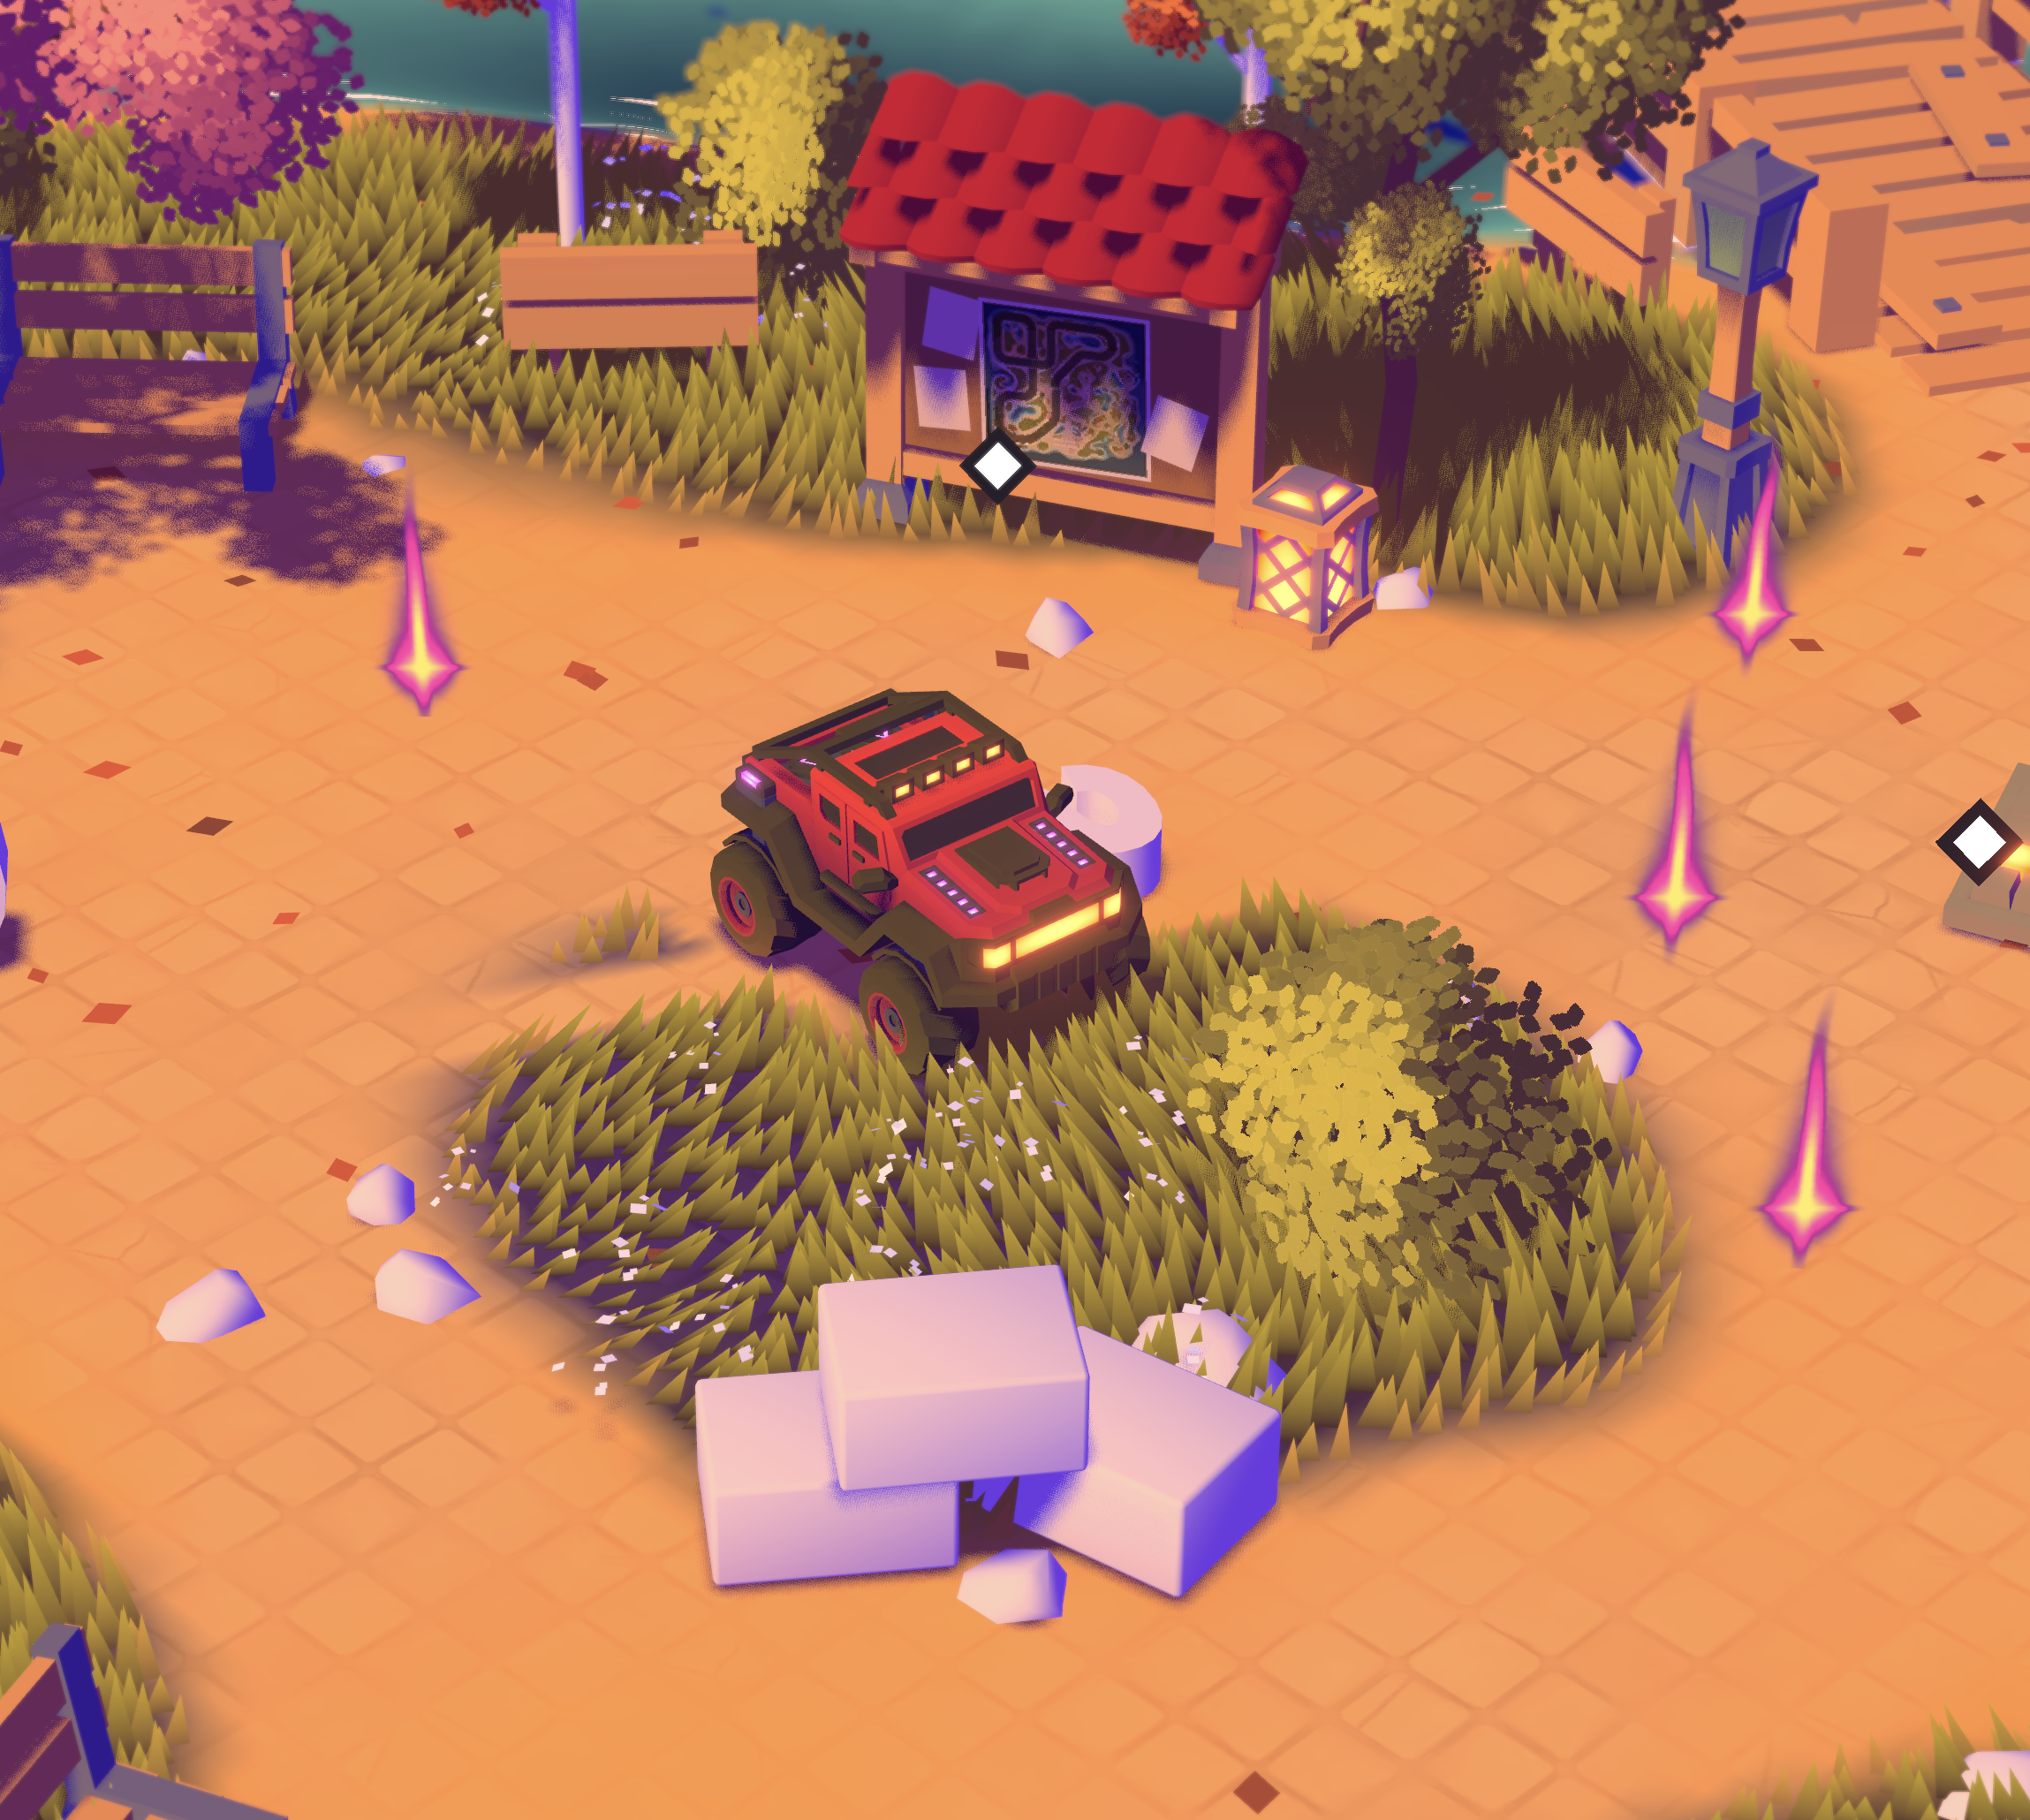
\includegraphics[width=.4\linewidth]{content/00_assets/threejs_portfolio_simon_bruno.png}
    \label{fig_threejs_portfolio_simon_bruno}
\end{figure}

Ebenso können mithilfe von ThreeJs komplette VR-Anwendungen im Browser umgesetzt werden. Die primäre Programmiersprache von ThreeJs ist JavaScript. Jedoch können auch darauf aufbauende Sprachen mit statischer Typisierung wie TypeScript\footnote{\url{https://www.typescriptlang.org/}} ohne Probleme verwendet werden. 

\subsection{BabylonJs}
Nebst ThreeJs ist auch Babylon ein sehr prominentes webbasiertes Framework. BabylonJs wurde im Jahr 2013 von Microsoft und basiert auf der Programmiersprache TypeScript. Wie ThreeJs unterstützt auch BabylonJs sowohl WebGL2 als auch WebGPU. Das Framework hat im Gegensatz zu ThreeJs eine integrierte Physik-Engine, Inspektor (siehe Abbildung \ref{fig_babylonjs_inspektor}) sowie einen Editor um UI Elemente zu gestalten \parencite{babylonjs_gui_editor_2025}. All diese Features machen BabylonJs zu einem populären Webframework welches rund 14'600 mal pro Woche heruntergeladen wird \parencite{babylonjs_npm_2025}. Die Downloadgrösse beträgt hierbei rund 60MB und ist somit rund doppelt so gross wie jene von ThreeJs. Wie ThreeJs hat auch BabylonJs eine umfassende Dokumentation\footnote{\url{https://doc.babylonjs.com/}}. Im Gegensatz zu ThreeJs welches einen modularen Aufbau bevorzugt, gibt BabylonJs in vielen Bereichen die Struktur und Art und Weise vor, wie ein Problem zu lösen ist \parencite{babylonjs_vs_threejs_2025}. BabylonJs ist ebenfalls ein Open Source Framework und kann daher kostenfrei verwendet werden. Aufgrund der Apache 2.0 Lizenz kann das Framework zudem ohne Bedenken für kommerzielle Zwecke eingesetzt werden \parencite{babylonjs_lizenz_2025}.
\begin{figure}[H]
    \caption{BabylonJs Inspektor \parencite{babylonjs_inspector_2025}}
    \includegraphics[width=.4\linewidth]{content/00_assets/babylonjs_inspektor.png}
    \label{fig_babylonjs_inspektor}
\end{figure}

\subsection{Sokol}
Nebst dem Browser gibt es natürlich auch native Applikationen, welche direkt auf dem Betriebssystem komplett ohne Browser laufen. Jedes Betriebssystem verwendet hierbei jedoch eine andere Grafikschnittstelle. Windows verwendet beispielsweise DirectX, Linux benutzt OpenGL/Vulkan und MacOS Metal. Wenn also eine Applikation auf allen Betriebssystemen laufen soll, dann muss pro Grafikschnittstelle eine Anwendung geschrieben werden, welche mit der entsprechenden Grafikschnittstelle interagiert. Sokol\footnote{\url{https://github.com/floooh/sokol}} ist ein Framework, welches verschiedene Grafikschnittstellen abstrahiert und vereinheitlicht. Dies hat den Vorteil, dass die Anwendung mit einem Framework wie Sokol nur einmal entwickelt werden muss. Sokol selbst ist ebenfalls Open Source unter der Zlib Lizenz und kann daher bedenkenlos für kommerzielle Projekte eingesetzt werden. Sokol ist in der systemnahen Programmiersprache C geschrieben und daher besonders performant und ressourcenschonend. Es stehen diverse Tools zur Verfügung, welche das Arbeiten mit 3D-Grafikschnittstellen vereinfachen. Das Shader Code Generator Tool\footnote{\url{https://github.com/floooh/sokol-tools/blob/master/docs/sokol-shdc.md}} (sokol-shdc) erlaubt es beispielsweise, Shader für verschiedene Schnittstellen zu generieren (eine Erklärung zu Shader folgt in Kapitel \ref{chap_render_pipelines}). Nebst den bekannten Betriebssytemen unterstützt Sokol zudem den Browser als Zielplattform. Hierzu wird \acrfull{Wasm} verwendet um C-Code in eine Assembler ähnliche Sprache für den Browser zu übersetzen. \acrshort{Wasm} hat den Vorteil, dass der generierte Code eine geringe Dateigrösse aufweist und performant ist. Sokol sebst steht als Single-header C Bibliothek zur Verfügung. Das bedeutet, dass sich der gesamte Code für eine Funktionalität in einer einzelnen Datei befindet. Dies erleichtert die Integration in ein bestehendes Projekt, da nur jeweils eine Datei integriert werden muss und kein komplexes Build-System notwendig ist. Die Dokumentation selbst befindet sich bei Sokol ebenfalls in den entsprechenden Dateien und ist in Form von Quellcode-Kommentaren vorhanden. Ebenfalls stehen mithilfe von \acrshort{Wasm} diverse Beispiele inkl. Beispielcode online zur Verfügung (siehe Abbildung \ref{fig_sokol_beispiele}).
\begin{figure}[H]
    \caption{Sokol Onlinebeispiele \parencite{sokol_beispiele_2025}}
    \includegraphics[width=.6\linewidth]{content/00_assets/sokol_beispiele.png}
    \label{fig_sokol_beispiele}
\end{figure}

\subsection{Electron}
Es wurden sowohl webbasierte als auch native Frameworks thematisiert. Webbasierte Frameworks haben im Gegensatz zu den nativen Frameworks den Vorteil, dass keine Installation notwendig ist und sie auf einem breiten Spektrum von Endgeräten lauffähig sind. Der Nachteil von webbasierten Frameworks abgesehen von der grösseren Ressourcenauslastung, liegt auch beim eingeschränkten Zugriff auf Dinge wie Multithreading sowie auf das Dateisystem. Electron\footnote{\url{https://www.electronjs.org/}} ist ein Framework, welches browserbasierten Anwendungen erlaubt, nativ auf dem Betriebssystem ausgeführt zu werden. Hierzu verpackt Electron einen Chromium basierter Browser sowie eine NodeJs Runtime in die native Anwendung \parencite{electron_documentation_2025}. Hierdurch steigt der eigentliche Festplattenverbrauch da neben der eigentlichen browserbasierten Anwendung noch ein kompletter Browser (Chromium) und eine JavaScript-Laufzeitumgebung (NodeJs) mitausgeliefert wird, jedoch können so Browseranwendungen nativ auf dem Betriebssystem laufen und Zugriff auf diverse Funktionalitäten wie Dateisystem, Kamera etc. erhalten \parencite{electron_why_2025}. Electron ist ebenfalls Open Source und steht unter der sehr freizügigen MIT Lizenz sowohl für private als auch kommerzielle Projekte ohne Einschränkungen zur Verfügung \parencite{electron_license_2021}.

\subsection{Tauri}
Tauri\footnote{\url{https://v2.tauri.app/}} hat wie Electron das Ziel browserbasierte Anwendungen als native Applikationen auf dem Betriebssytem auszuführen. Anders als Electron verpackt Tauri jedoch nicht einen kompletten Browser in die native Anwendung. Viele Betriebssysteme besitzen eine eigene WebView um etwa browserbasierte Anwendungen in nativen Apps etc. darzustellen. WebViews sind leichtgewichtiger als Browser und sparen daher auch Festplattenspeicher. Eine Anwendung welche Tauri als Framework anstelle von Electron verwendet, kann somit auf bis zu 600KB reduziert werden. Viele Unternehmen wie Microsoft verwenden WebViews bereits in den eigenen Produkten wie Microsoft Teams \parencite{microsoft_teams_webview_2023}. Um auf native Betriebssystemfunktionalitäten zuzugreifen stehen verschiedene Module in der systemnahen Programmiersprache Rust zur Verfügung. Ein Nachteil von WebViews im Gegensatz zu kompletten Browsern wie Chromium besteht darin, dass Unterschiede in den angebotenen Funktionalitäten je nach Betriebssystem auftreten können. Wenn jedoch Festplattenspeicher wie auch eine ressourcenschonendere Anwendung im Vordergrund stehen, ist Tauri eine ansprechende Alternative zu Electron.

\section{Immersive Technologien}
Frameworks und Engines helfen dabei, ansprechende 3D-Erlebnisse zu gestalten. Um jedoch ein immersives Erlebnis zu gewährleisten, reicht das alleine nicht aus. Technologien wie \acrshort{VR} und \acrshort{CAVE}-Systeme helfen dabei, die Immersion für den Nutzer komplett zu machen und ihm das Gefühl zu vermitteln, dass er sich mitten in der virtuellen Welt befindet.

\subsection{\acrfull{VR}}
Bei klassischen 3D Anwendungen befindet sich der Nutzer in der Regel vor einem Bildschirm oder einem Smartphone. \acrshort{VR} funktioniert anders. Anstelle eines Bildschirms wird ein \acrshort{VR}-Headsets sowie entsprechende Controller verwendet (siehe Abbildung \ref{fig_vr_headset_controller}). Dies sorgt für ein besonders immersives Erlebnis. Mithilfe der Controller kann der Nutzer sich durch die virtuelle Welt bewegen und kann mithilfe des Headsets den Kopf und die Blickrichtung komplett frei bestimmen. Jedoch muss entsprechend viel Bewegungsfreiraum vorhanden sein. Zudem müssen die Geräte entsprechend kalibriert werden. Moderne Browser und Webframeworks wie ThreeJs sowie BabylonJs erlauben es ebenfalls, VR-Anwendungen direkt innerhalb des Browsers mithilfe der WebXR\footnote{\url{https://immersiveweb.dev/}}-API umzusetzen. VR-Anwendungen sind somit nicht nur auf native Plattformen und mobile Endgeräte beschränkt und erhalten eine noch breitere Reichweite und Adaption.
\begin{figure}[H]
    \caption{Person mit VR-Headset und Controller \parencite{vr_headset_controller}}
    \includegraphics[width=.6\linewidth]{content/00_assets/vr_headset_controller.jpg}
    \label{fig_vr_headset_controller}
\end{figure}

\subsection{\acrfull{CAVE}}
Anders als bei \acrshort{VR} ist bei einem \acrshort{CAVE}-System kein Headset notwendig. Für ein CAVE-System benötigt es einen Raum, in dem sich der Nutzer frei bewegen kann. Auf den Wänden des Raums werden projektierte Bilder dargestellt \parencite{cave_1992}. Dies gibt den Nutzern das Gefühl, dass sie sich inmitten der Visualisierung befinden. CAVE macht es im Gegensatz zu VR einfacher mit verschiedenen Personen zu kollaborieren. Mehrere Personen können gleichzeitig in einem Raum sein und miteinander über wichtige Aspekte der Visualisierung diskutieren (siehe Abbildung \ref{fig_cave_collaboration}). 
\begin{figure}[H]
    \caption{Kollaboration in einem CAVE-System \parencite[S. 11]{cave_collaboration_2020}}
    \includegraphics[width=.6\linewidth]{content/00_assets/cave_collaboration.png}
    \label{fig_cave_collaboration}
\end{figure}

Dies ist vor allem im Bildungsbereich und in wissenschaftlichen Visualisierungen ein grosser Vorteil \parencite{cave_collaboration_2020}. Jedoch sind auch die Anschaffungskosten eines CAVE-Systems im Vergleich zu VR höher. Es braucht mehrere Projektoren sowie entsprechende Hardware. Für die CAVE-Anwendung selbst wird ebenfalls entsprechende Software benötigt, welche die 3D-Visualisierung verzerrungsfrei und synchron auf alle entsprechenden Wände projiziert. Hierzu wird das Master-Slave Prinzip angewendet. Pro Wand gibt es einen entsprechenden Rechner und Projektor. Auf jedem Rechner läuft die gleiche Visualisierung. Einer der Rechner (Master) gibt den Takt zur Synchronisierung vor und übermittelt die notwendigen Synchronisationsdaten (Kameraposition etc.) an die anderen Rechner (Slave). Ein CAVE-System kann mit entsprechender Hardware beliebig erweitert werden. Beispielsweise erlauben Headtracker das dynamische Verfolgen der Person im Raum. Hiermit kann die 3D-Visualisierung sich entsprechend an Hand der 3D Position der Personen anpassen. Aufgrund des breiten Spektrums der Erweiterungsmöglichkeiten ergeben sich auch unterschiedliche Preissegmente, angefangen bei vierstelligen bis hin zu siebenstelligen Beträgen. Für das Bereitstellen solcher Räume gibt es auch spezialisierte Firmen wie Inside Reality\footnote{\url{https://inside-reality.com/product/icroom/}}, welche nebst der entsprechenden Software auch die entsprechende Hardware und den Aufbau hierzu anbieten.